\documentclass{article}
\usepackage[french]{babel}
\usepackage[T1]{fontenc}

\usepackage{graphicx} % Required for inserting images
\graphicspath{{ressources/}}
\usepackage{csquotes}
\usepackage[hyphens]{url}
\usepackage{amsmath}
\usepackage{amsfonts}
\usepackage{fancyhdr}
\usepackage{biblatex}
\addbibresource{Attracteur de Lorenz.bib}

\usepackage{thmbox}

\usepackage{tikz}
\usepackage[firstpage = True]{background}
\usepackage{array}
\usepackage{epigraph}

\pagestyle{fancy}
\fancyhead{}
\fancyfoot{}
\fancyhead[L]{Attracteur de Lorenz - \thesection}
\fancyhead[R]{
\includegraphics[height =15pt]{logoUPS}}
\setlength{\headheight}{20pt}
\fancyfoot[C]{\thepage}

\title{Système de Lorenz}

\setlength \epigraphwidth {0.4\linewidth}
\AtBeginDocument{\renewcommand {\epigraphflush}{center}}
\renewcommand {\sourceflush} {center}

\newcommand*\colv[1]{
\left(\begin{array}{c}
    #1
\end{array}\right)
}

\newcommand{\R}{\mathbb{R}}

\newcommand{\deriv}[3][ ]{
    \ensuremath{\frac{\mathrm{d}^{#1}#2}{\mathrm{d}^{#1} #3}}
}
\newcommand{\id}[1][]{\ensuremath{\mathrm{Id}_{#1}}}

\newcommand{\cad}{c'est-\`a-dire }

\newcommand{\setbackground}[1]{ \backgroundsetup{ scale=1, opacity=1, angle=0, contents={ \includegraphics[width=\paperwidth]{#1} } } }

\newtheorem[M , nocut]{prop}{Proposition}[section]
\newtheorem[M , nocut]{definition}{Définition}
\newtheorem[M , nocut]{lemme}{Lemme}
\newtheorem[L , nocut]{thm}{Théoreme}
\newtheorem[M , nocut]{cor}{Corollaire}

\begin{document}
\begin{titlepage}
    \BgThispage
    \setbackground{LorenzTransparentbis}
    \clearpage
    \begin{center}
        \vspace{1cm} 
        \Huge
        \textbf{Attracteur de Lorenz}\\
        \vspace{0.5cm}
        \Large
        Projet de licence 3\\
        \vspace{1.5cm}
            
        \textbf{Adrien CHABERT\\Louka OUKALA\\Salome COUDIERE}    
        \vfill
        Second semestre - Année 2023-2024
    \end{center}
\end{titlepage}
\newpage
\hfill
\thispagestyle{empty}
\newpage

\thispagestyle{empty}
\vspace*{\fill}
\epigraph {\centering Je me rature ardemment. \\ Il faut n'écrire que le strict nécessaire.} {— Claude NOUGARO}
\vspace*{\fill}
\newpage

\thispagestyle{empty}
\vspace*{\fill}
Nous tenons à remercier, notre professeur référent pour ce projet M. Filbet, pour le temps s'il a consacré à nous apprendre la méthodologie pour rédiger ce mémoire. La rigueur exigée sera un atout dans la poursuite de nos études.\\
Nous remercions aussi l'ensemble de nos professeurs qui s'efforce de nous transmettre leur précieux savoir.\\
Je tiens aussi à remercier mon père pour avoir relu et corriger ce document ainsi que pour son soutien indéfectible.
\vspace*{\fill}
\newpage
\tableofcontents
\thispagestyle{empty}
\newpage

\section{Introduction}
\thispagestyle{empty}
\setcounter{page}{1}
\begin{quotation}
    Does a flap of a butterfly's wings in Brazil set off a tornado in Texas?
\end{quotation}
C'est le titre de l'article que Edward N. Lorenz publie en 1972 \cite{edward_lorenz_does_1972}, dans le quel il fait la synthèse de ce que l'on connait sous le nom de la théorie du chaos. La question peut être traduite par "Est-ce qu'un battement d'ailes de papillon au Brésil peut entrainer une tornade au Texas ?". En effet lors de l'étude de certains systèmes, une faible variation peut entraîner des changements considérables dans les états ultérieurs du système. Tout au long de sa vie Lorenz se sera intéressé aux systèmes chaotiques essentiellement appliqués à son domaine de recherche : la météorologie. Dès 1963, il propose un modèle simplifié pour essayer de décrire la méteo \cite{edward_n_lorenz_deterministic_1963}. Ce modèle a contribué à montrer la difficulté de prédire le climat sur le long terme. Ce modèle a été présenté sous la forme suivante.
\begin{equation}
    \label{Lorenz}
    \left\{
    \begin{array}{rl}
        x' &=\sigma(y-x), \\
        y' &=\rho x -y - xz,\\
        z' &=xy - \beta z,
    \end{array}
    \right.
    \begin{array}{r}
        (L_1)\\
        (L_2)\\
        (L_3)
    \end{array}
\end{equation}
(\textit{Avec $\sigma,\rho,\beta$ des paramètres}). Dans ce système les inconues sont les fonctions du temps $t$, $x$,$y$ et $z$. L'indicateur $x$ des mouvements de convection, $y$ est proportionnel à la variation de température dans les courants verticaux, et $z$ est un indicateur de la variation de température par rapport à un profil linéaire. Dans l'approximation les paramètres $\sigma$ et $\rho$ correspondent au nombre de Prandtl et au nombre de Rayleigh. Nous nous interresseront uniquement à l'étude mathématique de ce système. Ce système est appelé l'attracteur de Lorenz (aussi appelé attracteur étrange ou système de Lorenz). \`A travers cette étude nous allons présenter certaines caractéristiques chaotiques du système en modélisant les résultats théoriques avec des applications numériques, nous pourrons notamment observer les courbes qui prennent la forme d'ailes de papillon qui donneront leur nom a l'effet éponyme.
   
\newpage
\section{Résultats fondamentaux pour les équations différentielles}

\subsection{Définitions}
Dans ce chapitre on rappelle les résultats sur lesquels repose notre étude.
\begin{definition}
    On appele équation différentielle une équation de la forme
    \[
      u'(t) = f(t,u(t))  
    \]où $f \in C(I\times U,\R^d)$ et $u \in C^1(I,U)$ avec $I$ un intervalle de $\R$ et $U \subset \R^d$ ouvert.
\end{definition}
\begin{example}[Remarque]
    Si $f$ ne dépend pas directement de $t$, l'équation est dite autonome
\end{example}
Lorsque l'on s'intéresse aux équations différentielles, on s'intéresse plus particulièrement au problème de Cauchy, que l'on peut définir comme suit.
\begin{definition}
    On appele problème de Cauchy, une équation différentielle munit d'une condition initiale (une information sur une valeur de la fonction). On le présente sous la forme d'un système.
    \[ \left\{ \begin{array}{l}
        u'(t) = f(t,u(t)) \\ 
        u(t=t_i) = u_i
    \end{array}\right. \]
    Avec $t_i\in I, u_i \in U$
\end{definition}

\subsection{Outils pour les équations différentielles}

Lorsque l'on souhaite étudier les équations différentielles le lemme de Grönwall est un outil essentiel, il permet notamment d'obtenir un contrôle sur le comportement des solutions.
\begin{lemme}
    \label{lemme:Gronwall}
    Soient $u\in C^1([0,T],\R_+)$ et $a\in C([0,T],\R)$ telles que:
    \[
      \forall t \in [0,T] u'(t)\le a(t)u(t)  
    \]Alors $\forall t \ge t_0, t_0 \in [0,T]$, on a:
    \[
        u(t) \le u(t_0)e^{\int_{t_o}^t a(s)\ \mathrm{d}s}
    \]
\end{lemme}
Cet énoncé du lemme n'est pas le plus complet qu'il est possible d'établir, il est cependant suffisant pour notre étude. On admet la démonstration que l'on peut retrouver dans le livre de Berthelin (p.18) \cite{florent_berthelin_equations_2021}.
L'outil le plus important pour l'étude des équations différentielles ordinaire, qui nous permet de déterminer l'existence et l'unicité des solutions est le théorème suivant.
\begin{thm}[Cauchy-Lipschitz]
    \label{thm:CL}
    Soient $f\in C(I\times U, \R^d)$ où $I$ est un intervalle de $\R$ et $U$ un ouvert de $\R^d$, et $(t_0,u_0)$. On suppose que $f$ est localement Lipschitzienne par rapport à la seconde variable sur $[0,T]$. Alors 
    \begin{itemize}
        \item il existe $T>0$ et $u\in C^1([0,T],U)$ est solution du problème de Cauchy
        \item si $v$ est une autre solution, elle coïncide avec $u$ sur l'intervalle $[0,T]$
    \end{itemize}
\end{thm}
Nous admettrons la démonstration de ce théorème dont on peut retrouver dans le livre de F. Filbet (section 6.2.2) \cite{francis_filbet_analyse_2009}.
Maintenant que nous avons introduit les principaux outils pour l'étude des équations différentielles, on peut à présent s'interresser au système de Lorenz \eqref{Lorenz}

\newpage
\section{Existence et premières propriétés}

Dans cette section nous allons faire une étude du systeme de Lorenz afin de déterminer l'existence des solutions. Nous nous limiterons à l'étude des temps positifs ($t \ge 0$).

\begin{prop}
    Le système de Lorenz admet une unique solution sur $\R_+$ de classe $C^1$
\end{prop}

\begin{proof}
    Premièrement, on transforme le système de Lorenz sous la forme d'un problème d'ordre 1.
    \begin{equation}
        \label{fLorenz}
        \deriv{\Vec{u}}{t} = \Gamma(\Vec{u}), \quad
        \Gamma : \Vec{u} = \colv{x\\y\\z} \in \R^3 \mapsto \colv{\sigma(y-x) \\ \rho x-y-xz \\ xy-\beta z}
    \end{equation}
     \`A présent montrons l'existence des solutions de ce système. $\Gamma$ est $C^1$ donc elle est localement Lipschitzienne, de plus elle ne dépend pas directement du temps. D'après le théorème de Cauchy-Lipschitz, l'équation \eqref{Lorenz} admet une unique solution de classe $C^1$ sur $[0,T]$ que l'on notera $(I,(x,y,z))$ avec $I \subset \R_+$ et $I = [0,T[,\ T \in ]0,+\infty]$. Montrons que $T = +\infty$. Dans \eqref{Lorenz} on s'intéresse à la somme de, $x$ fois première ligne avec $y$ fois la seconde ligne et $z$ fois la troisième ligne.
\[
    xx'+yy'+zz' = \sigma yx - \sigma x^2 + \rho xy - y^2 -xyz + xyz - \beta z^2\\
\]  
Posons $\mathcal{N}: (x,y,z) \in \mathcal{F}(\R,\R^3) \mapsto x^2 + y^2 + z^2$, c'est la norme euclidienne au carré. 

\begin{align*}
    \Rightarrow \frac{1}{2}\deriv{ }{t}\mathcal{N}(t) & =(\sigma + \rho)x(t)y (t) -\sigma x^2(t) - y^2(t) - \beta z^2(t)\\
    & \le (\sigma + \rho)x(t)y(t) +\min (1,\sigma,\beta)\mathcal{N}(t)\\
    & \le (\frac{\sigma+\rho}{2})(x^2(t) + y^2(t)) +\min (1,\sigma,\beta) \mathcal{N}(t) &&\mathit{(Young)}\footnotemark \\
    & \le (\frac{\sigma+\rho}{2})(x^2(t) + y^2(t) + z^2(t)) +\min (1,\sigma,\beta) \mathcal{N}(t)\\
    & \le \bigg[\frac{\sigma + \rho}{2} + \min (1,\sigma,\beta) \bigg] \mathcal{N}(t)
\end{align*}
\footnotetext{$\forall p,q \in \mathbb{N}\: \text{tels que} \frac{1}{p}+\frac{1}{q}=1 \Rightarrow \forall a,b \in \R \: ab \le \frac{a^p}{p}+\frac{b^q}{q}$}

Posons $ \eta = \sigma + \rho + 2 \min (1,\sigma,\beta)$. On a alors: 
\[
    \forall t \in \R_+, \  \deriv{}{t}\mathcal{N}(t) \le \eta\  \mathcal{N}(t)
\]
D'après le lemme de Grönwall il vient:
\[
    \forall t \in \R_+,\  \mathcal{N}(t) \le \mathcal{N}_0 e^{\eta t},\  \textrm{avec } \mathcal{N}_0 = \mathcal{N}(0)
\]
Donc la norme du vecteur solution n'explose pas en temps fini.
\end{proof}

En ayant obtenu les résultats de cette proposition, on peut aisément en déduire la propriété suivante.

\begin{cor}
    Les solutions du système de Lorenz \eqref{Lorenz} sont de classe $C^\infty$
\end{cor}

\begin{proof}
    Par \eqref{fLorenz} on a que $(x',y',z') = \Gamma(x,y,z)$, or par composition $\Gamma(x,y,z)$ est $C^1$ donc $(x',y',z')$ l'est aussi, ainsi $(x,y,z)$ est $C^2$. De la même manière on obtient par récurence immédiate que $(x,y,z)$ est $C^\infty$
\end{proof}

Cette propriété nous permet de dire que même si \eqref{Lorenz} est un système dit chaotique, on peut affirmer que les solutions sont régulières.

\newpage
\section{\'Etude des points stationnaires}

Après une première étude du système de Lorenz \eqref{Lorenz}, on s'intéresse maintenant à la stabilité du système de Lorenz autour des points d'équilibre que l'on définit comme suit.

\begin{definition}
    Soit $f\in C(U,\R^d)$ avec $U$ ouvert de $\R^d$, $f$ définit une équation différentielle autonome.
    On appele point stationnaire ou d'équilibre de l'équation différentielle, tout point $v \in U$ tel que:
    $$ f(v) = 0$$ 
\end{definition}

\subsection{Rappel des théorèmes}
\label{sec:Rappel-des-théorèmes}
Avant de s'intéresser aux théorèmes qui nous donnent les résultats de stabilité, on rappelle les définitions de la différentielle et du spectre qui nous serviront par la suite.
\begin{definition}
    Soient $f:U\subset \R^d \to \R^d$ et $a\in U$. On dit que $f$ est différentiable en $a$ s'il existe une application linéaire $L:\R^d\to\R^d$ telle que:
    $$f(a+h) = f(a) + L(h) + \|h\|\varepsilon(h)\quad \text{avec }\varepsilon(h)\xrightarrow[h\to 0]{}0$$ 
    L'application linéaire $L$ est alors appelée la differentielle de $f$ en $a$, on la note $\mathcal{D}_f(a)$
\end{definition}
\begin{example}[Remarque]
    Dans la suite on appellera différentielle, l'application linéaire et la matrice associée à l'application linéaire dans la base cannonique sans distinction.
\end{example}
\begin{definition}
    On définit le spectre d'une application linéaire $f$ sur un $\mathbb{K}-$espace vectoriel (avec $\mathbb{K}$= $\R$ ou $\mathbb{C}$).Comme l'ensemble des valeurs propres de $f$. On le note $\mathrm{Sp}(f)$
\end{definition}

Maintenant on rappelle les résultats sur lesquels on s'appuira dans la suite. Ces théorèmes établissent des résultats de stabilité dite linéaire autour des points stationnaires en se basant sur l'étude spectrale de la différentielle.
\begin{thm}
    \label{thm:eq-ass-stable}
    Soit $f\in C^2(U;\R^d)$ sur un ouvert $U$ de $\R^d$ et $v\in U$ tel que $f(v)=0$. Si le spectre de $\mathcal{D}_\Gamma(v)$ est inclus dans le demi-plan ouvert $\left\{\lambda; \Re(\lambda)<0\right\}$ alors $v$ est un point d'équilibre assymptotiquement stable pour l'équation $u'=f(u)$
\end{thm}

Ce résultat nous permet de conclure sur le comportement assymtotique des solutions ayant subit une faible perturbation à l'instant de départ. Ainsi deux solutions proche d'un point d'équilibre, une ayant subit une perturbation à l'instant initial et l'autre non, approchent assymptotiquement la même trajectoire.

\begin{thm}
    \label{thm:eq-instable}
    Soit $f\in C^2(U;\R^d)$ et $v\in U$ tel que $f(v)=0$. Si $\max\{\Re(\lambda); \lambda\in \mathrm{Sp}(\mathcal{D}_f(v))\}$ est atteint pour une valeur propre de $\mathcal{D}_f(v)$ de partie réelle strictement positive. Alors $v$ est un point d'équilibre instable pour l'équation $u'=f(u)$
\end{thm}

% commentaire sur le résultat

Ces théorèmes nous donnent des résultats seulemment pour des valeurs propres strictement négative ou strictement positive. Cependant ces théorèmes ne nous permettent pas de conclure sur le cas où $0$ est valeur propre de la différentielle. Il existe des résultats qui permettent de conclure sur la stabilité simple ($0$ valeur propre de la différentielle), cependant nous ne traiterons pas ce cas dans notre étude.

\subsection{Détermination des équilibres}
Dans un premier temps on regarde si notre système possède des équilibres, et si oui, lesquels.
\begin{prop}
    Si $\beta(1-\rho) \ge 0$, l'équation \eqref{Lorenz} possède 3 points d'équilibre qui sont:
    \begin{align*}
        S_0 := 0_{\R^3} &&   S_+ :=\colv{\sqrt{ \beta (\rho -1)} \\ \sqrt{\beta (\rho -1)}\\ \rho -1}  &&  S_- := \colv{-\sqrt{ \beta (\rho -1)} \\ - \sqrt{\beta (\rho -1)}\\ \rho -1}
    \end{align*}
\end{prop}

\begin{proof}
On remarque que $(0,0,0)$ est un point stationnaire, en effet $\Gamma(0,0,0) = 0_{\R^3}$ donc ($\R_+$,$0_{\R^3}$) est une solution de l'équation différentielle.\\
On résout alors $\Gamma(x,y,z)=0_{\R^3}$ en supposant que $(x,y,z) \neq 0_{\R^3}$, il vient:
\[
\left\{\begin{array}{rl} %O of Gamma
     \sigma(y-x)&=0  \\
     \rho x -y -xz&=0\\
     xy - \beta z&=0
\end{array}\right.
\begin{array}{c} %Num eq
    (L_1)\\
    (L_2)\\
    (L_3)
\end{array}
\]
de $(L_1)$ on obtient que $x=y$. Dans $(L_2)$ et dans $(L_3)$ on remplace $y$ par $x$, il vient alors:
\begin{gather*}
    (L_2) \Rightarrow \rho x - x - xz = 0 \Rightarrow x (\rho -1 -z ) = 0 \\
    (L_3) \Rightarrow x^2 - \beta z = 0 \Rightarrow z = \frac{x^2}{\beta}
\end{gather*}
On obtient ainsi un polynôme de degré 3, il y a donc au plus 3 équilibres:
\begin{align*}
    (L_2) & \Rightarrow x (\rho - 1 - \frac{x^2}{\beta}) = 0 \text{, or }x \neq 0\\
        & \Rightarrow x^2 = \beta (1-\rho)\\
    \text{Si } \beta(1-\rho) \ge 0 & \Leftrightarrow \beta \ge 0,\rho\le 1 \text{ ou } \beta \le 0,\rho\ge 1\text{ alors:}\\
    &\Rightarrow x = \pm \sqrt{\beta(1-\rho)}
\end{align*}

De ces trois équations on obtient que:
\[
    \Gamma(x,y,z)=0_{\R^3} \Rightarrow (x,y,z) = (\pm \sqrt{ \beta (\rho -1)} ,\pm \sqrt{\beta (\rho -1)}, \rho -1)
\]

On vérifie aisément que cette relation est une \'equivalance, en remplaçant les valeurs obtenues de $x$,$y$ et $z$ dans $\Gamma(x,y,z)$
\end{proof}

\begin{example}[Remarque]
    Si $\rho=1, 0$ est une racine triple de $\chi$, donc $0_{\R^3}$ est un point stationnaire triple pour \eqref{Lorenz}.
\end{example}

\subsection{Stabilité de l'équilibre $0_{\R^3}$}
Afin d'utiliser les outils introduits dans la partie \ref{sec:Rappel-des-théorèmes}, on présente le lemme suivant.
\begin{lemme}[préliminaire]
    Le polynôme caractéristique de la différentielle de $\Gamma$ évalué en $0_{\R^3}$ est:
    $$ \chi(\lambda) = (\lambda + \beta)P(\lambda)$$
    Avec $P:\lambda \in \R \mapsto \lambda^2 + \lambda(\sigma+1)+\sigma-\rho\sigma$, de plus le discriminant de P est:
    $$ \Delta = (\sigma-1)^2 +4\sigma\rho $$
    Notons que $-\beta$ est toujours racine de $\chi$
\end{lemme}

\begin{proof}
Dans un premier temps on calcule la différentielle de $\Gamma$:
\begin{equation}
    \label{eq:diff}
    \mathcal{D}_\Gamma(x_s,y_s,z_s) = 
    \left(\begin{array}{ccc}
        -\sigma & \sigma & 0\\
        \rho- z_s & -1 & -x_s\\
        y_s & x_s & -\beta
    \end{array}\right)
\end{equation}

A présent, on calcule le polynôme caractéristique de la différentielle en $0_{\R^3}$ (noté $\chi$) donné par le calcul suivant.
\[
    \chi (\lambda) = \det\big(\lambda\id - \mathcal{D}_{\Gamma}(0,0,0)\big) = (\lambda + \beta)(\lambda^2 + \lambda(\sigma+1)+\sigma-\rho\sigma)
\]
Posons $P$ comme dans le lemme. Ainsi pour étudier $\chi$, on calcule le discriminant de $P$:
\[
  \Delta = (\sigma+1)^2 - 4(\sigma-\sigma\rho) = (\sigma-1)^2 +4\sigma\rho
\]
\end{proof}

Dans l'étude que l'on propose on va distinguer trois cas pour étudier la stabilité de l'équilibre du système de Lorenz près de l'origine.
\begin{figure}[ht]
    \centering
    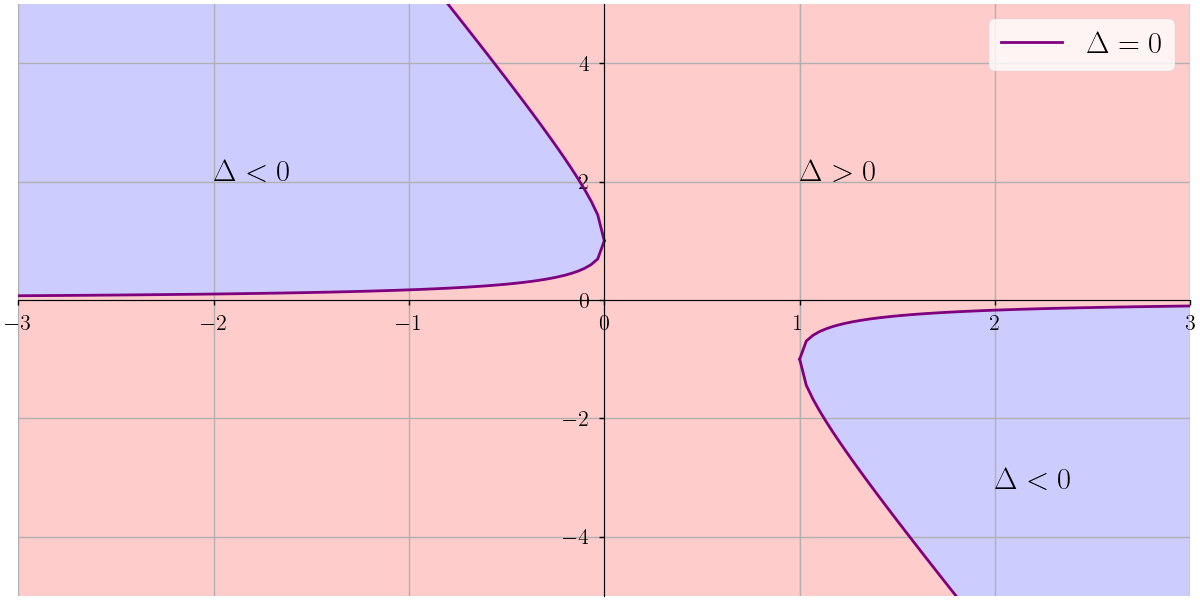
\includegraphics[width=0.8\textwidth]{DeltaDomain}
    \caption{Signe de $\Delta$ en fonction de $\rho$ en abscisse et de $\sigma$ en ordonnée}
    \label{fig:signD}
\end{figure}


\subsubsection*{Cas $\Delta > 0$}
\addcontentsline{toc}{subsubsection}{\protect\numberline{} Cas $\Delta>0$}

\begin{prop}
    \label{prop:eqDsup0}
    Dans le cas $\Delta>0$ si $\beta<0$ l'équilibre $0_{\R^3}$ est instable, si $\beta >0$ on a :
    \begin{itemize}
        \item Si $\sigma(\rho-1)>0$ alors $0_{\R^3}$ est un équilibre instable pour \eqref{Lorenz}
        \item Si $\sigma(\rho-1)<0$ alors $0_{\R^3}$ est un équilibre assymptotiquement stable pour \eqref{Lorenz}
    \end{itemize}
\end{prop}

\begin{proof}
    Premièrement, on détermine les conditions pour que $\Delta$ soit strictement positif.
    \begin{lemme}
        $\Delta$ est strictement positif pour l'ensemble des paramètre suivant:
        \[
         \left\{(\sigma,\rho)\in \R ^2 : 1-2 \rho - \sqrt{\frac{(4\rho-2)^2}{4} -1 } > \sigma\ ou \ \sigma > 1-2 \rho + \sqrt{ \frac{(4\rho-2)^2}{4} -1  } \right\}    
        \]
    \end{lemme}
    
        \begin{proof}[(Lemme)]
            $\Delta = \sigma^2 + \sigma(4\rho-2) + 1$ est un polynôme de la variable $\sigma$. On note le déterminant de $\Delta$ selon la variable $\sigma$, $\delta$. $\Delta$ est convexe par rapport à la variable $\sigma$ donc $\Delta$ est strictement positif à l'extérieur de ses racines. On a donc:
            \begin{align*}
                \sigma <& 1-2 \rho - \sqrt{\frac{(4\rho-2)^2}{4} -1 }\\
                \text{ou}\\
                \sigma >& 1-2 \rho + \sqrt{\frac{(4\rho-2)^2}{4} -1 }
            \end{align*}
            %finir demo !
        \end{proof}
        
    Maintenant regardons l'équilibre $0_{\R^3}$ dans le cas $\Delta> 0$. On peut expliciter les racines de $\chi$ qui constitue le spectre de la différentielle de $\Gamma$. On a ainsi:
    \[
        \mathrm{Sp}(\mathcal{D}_\Gamma (0_{\R^3}))= \left\{-\beta,\lambda_+ := \frac{-(\sigma+1) + \sqrt{\Delta}}{2},\lambda_- := \frac{-(\sigma+1) - \sqrt{\Delta}}{2}\right\}  
    \]

    Premièrement on différencie le cas $\beta<0$, dans ce cas alors, $\max(\mathrm{Sp}(\mathcal{D}_\Gamma (0_{\R^3})))\ge -\beta > 0$, donc dans ce cas $0_{\R^3}$ est un équilibre instable pour \eqref{Lorenz}. Dans le cas où $\beta$ est positif,comme $\lambda_+>\lambda_-$, si $\lambda_+ > 0$, l'équilibre est instable sinon l'équilibre est assymptotiquement stable. On cherche alors $\rho$ et $\sigma$ tel que $\lambda_+>0$
    \begin{align*}
        && \frac{-(\sigma+1) + \sqrt{(\sigma-1)^2+4\rho\sigma}}{2} &>0 \\
        \Leftrightarrow && (\sigma-1)^2+4\rho\sigma &> (\sigma+1)^2 \\
        \Leftrightarrow && \sigma(\rho-1) &> 0
    \end{align*}
\end{proof}


\subsubsection*{Cas $\Delta = 0$}
\addcontentsline{toc}{subsubsection}{\protect\numberline{} Cas $\Delta=0$}


\begin{prop}\label{prop:eqDeg0}
    Dans le cas $\Delta=0$:
    Si $\beta <0$ l'équilibre est instable si $\beta>0$ alors on a:
    \begin{itemize}
        \item Si $\sigma < -1 , \rho > 1$ alors $0_{\R^3}$ est un équilibre instable pour \eqref{Lorenz}
        \item Si $\sigma > -1 , \rho < 1$ alors $0_{\R^3}$ est un équilibre assymptotiquement stable pour \eqref{Lorenz}
    \end{itemize}
\end{prop}

\begin{proof} %DEMO
    On s'intéresse d'abord aux cas tels que $\Delta=0$

    \begin{lemme} 
        \label{lemme:Deg0}
        $\Delta$ est nul si et seulemment si on a la paramétrisation suivante,
        \[
            \left\{(\sigma,\rho)\in \R ^2 :\sigma = 1-2 \rho + \sqrt{ \frac{(4\rho-2)^2}{4} -1 }\ ou\ \sigma = 1-2 \rho - \sqrt{ \frac{(4\rho-2)^2}{4} -1 } \right\}  
        \]
        Cette paramétrisation implique que $\rho \in \R \setminus ]0,1[$
    \end{lemme}
    
    \begin{proof}[(Lemme)]
        A nouveau on considère $\Delta$ comme un polynôme de la variable $\sigma$. Pour que $\Delta$ ait des racines, il faut que $\delta$ soit positif ou nul.
        \[
        \delta \ge 0 \Leftrightarrow \rho(\rho-1) \ge 0 \Leftrightarrow \rho \in \R \setminus ]0,1[
        \] Maintenant on calcule les racines de $\Delta$.
        \begin{align*}
            \sigma &= \frac{2-4\rho + \sqrt{ (4\rho-2)^2 -4 }}{2} = 1-2 \rho + \sqrt{ \frac{(4\rho-2)^2}{4} -1 }\\
            \text{ou}\\
            \sigma &= \frac{2-4\rho - \sqrt{ (4\rho-2)^2 -4 }}{2} = 1-2 \rho - \sqrt{ \frac{(4\rho-2)^2}{4} -1 }
        \end{align*}
        On obtient ainsi la paramétrisation voulue.
    \end{proof}
    Maintenant on s'intéresse à la stabilité de l'équilibre dans le cas $\Delta=0$. Comme $-\beta$ est toujours racine de $\chi$ si $\beta <0$ alors $\max (\mathrm{Sp}(\mathcal{D}_\Gamma (0_{\R^3}))) \ge -\beta > 0$ donc d'après le théorème \ref{thm:eq-instable}, $0_{\R^3}$ est un équilibre instable pour \eqref{Lorenz}\\
    Si $\beta > 0$ alors dans le cas de $\Delta = 0, \mathrm{Sp}(\mathcal{D}_\Gamma) = \{\beta, -\frac{\sigma+1}{2}\}$, on cherche alors les conditions sur les paramètres $\sigma$ et $\rho$ telles que le système soit instable ou assymptotiquement stable.
    On s'intéresse au cas instable et on inversera le sens des inégalités pour avoir le cas assymptotiquement stable. 
    \[
        -\frac{\sigma+1}{2} >0 \Leftrightarrow \sigma < -1   
    \]
    Dans la première équation de la paramétrisation on obtient que 
    \[-1 > 1-2 \rho + \sqrt{ \frac{(4\rho-2)^2}{4} -1}\] n'a pas de solutions.\\
    Dans la seconde équation on cherche $\rho$ tel que:
    \[
        1-2 \rho - \sqrt{ \frac{(4\rho-2)^2}{4} -1 } < -1 \Rightarrow \frac{(4\rho-2)^2}{4} -1 > (2\rho-2)^2 \Leftrightarrow \rho > 1 
    \]En faisant les caluls avec l'inégalité inverse, on retrouve le cas assymptotiquement stable.
\end{proof}

\subsubsection*{Cas $\Delta < 0$}
\addcontentsline{toc}{subsubsection}{\protect\numberline{} Cas $\Delta<0$}

% Stabilité cas \Delta < 0
\begin{prop}
    \label{prop:eqDinf0}
    Dans le cas $\Delta<0$:
    Si $\beta <0$ l'équilibre est instable si $\beta>0$ alors on a:
    \begin{itemize}
        \item Si $\sigma < -1 , \rho > 1$ alors $0_{\R^3}$ est un équilibre instable pour \eqref{Lorenz}
        \item Si $\sigma > -1 , \rho < 1$ alors $0_{\R^3}$ est un équilibre assymptotiquement stable pour \eqref{Lorenz}
    \end{itemize}
\end{prop}
\begin{proof}
    On détermine les cas tels que $\Delta<0$
    %CAS \Delta < 0
    \begin{lemme}
        $\Delta$ est strictement négatif pour l'ensemble des paramètres suivants:
        \[
        \left\{(\sigma,\rho)\in \R ^2 : 1-2 \rho - \sqrt{ \frac{(4\rho-2)^2}{4} -1 }< \sigma < 1-2 \rho + \sqrt{ \frac{(4\rho-2)^2}{4} -1 } \right\}    
        \]Dans cet ensemble on a: $\rho \in \R \setminus [0,1]$ 
    \end{lemme}

    \begin{proof}[(Lemme)]
     Pour que $\Delta$ ait des racines, il faut que $\delta$ soit strictement positif.
    \[
    \delta > 0 \Leftrightarrow \rho(\rho-1) > 0 \Leftrightarrow \rho \in \R \setminus [0,1]
    \]Par convexité de $\Delta$ on a que $\Delta$ est négatif entre ses racines, il vient alors:
    \[
        1-2 \rho - \sqrt{ \frac{(4\rho-2)^2}{4} -1 } < \sigma < 1-2 \rho - \sqrt{ \frac{(4\rho-2)^2}{4} -1 }
    \]Donc l'ensemble des $\rho,\sigma$ qui vérifie cette inégalité sont alors des paramètres tels que $\Delta$ est négatif.
    \end{proof}

    On détermine les cas pour lesquels l'équilibre est instable ou assymptotiquement stable. Pour la différenciation du cas de $\beta$ cf. la démonstration de \ref{prop:eqDeg0}. Ainsi il vient:
    \[
        \mathrm{Sp}(\mathcal{D}_\Gamma (0_{\R^3})) = \left\{\beta, \omega := \frac{-(\sigma+1)+ i \sqrt{-\Delta}}{2}, \bar{\omega} := \frac{-(\sigma+1)- i \sqrt{-\Delta}}{2}\right\}
    \]Pour étudier la stabilité on s'intéresse à la partie réelle de $\omega$ et $\bar{\omega}$. Or $\Re (\omega) = \Re (\bar{\omega}) = -\frac{\sigma+1}{2}$ on retombe ainsi sur le même calcul que dans la démonstration de la propriété \ref{prop:eqDeg0}. On retrouve bien le cas voulu.
\end{proof}

\subsection{Stabilité de $S_\pm$}

Dans cette section nous allons nous intéresser aux points d'équilibres définit précédemment $S_+$ et $S_-$. Nous ferons aussi quelques hypothèses simplificatrices, supposons $\sigma,\rho,\beta$ positifs et de plus $\sigma>\beta+1$.

\begin{prop}
    Sous les hypothèses de cette section et si $\rho > 1$ alors on définit $\rho^* = \sigma \frac{\sigma+\beta+3}{\sigma-\beta-1}$ tel que 
    \begin{itemize}
        \item si $\rho < \rho^* $ alors les équilibres $S_\pm$ sont assymptotiquement stables pour \eqref{Lorenz}
        \item si $\rho > \rho^* $ alors les équilibres $S_\pm$ sont instables pour \eqref{Lorenz}
    \end{itemize}
\end{prop}

\begin{example}[Remarque]
    Si $\rho \in [0,1[$ les équilibres $S_\pm$ n'existent pas.
\end{example}

Nous admettrons le résultat ci-dessus, une démonstration est proposée dans la thèse de D. Jones \cite{daniel_jones_stability_2009}.

\newpage
\section{Méthodes numériques}

Dans cette section nous allons introduire les méthodes numériques pour la résolution d'équation différentielle ordinaire (EDO). 
\begin{example}[Problématique]
    Pourquoi introduire des méthodes numériques pour la résolution des EDO ? 
\end{example}
Lorsque on étudie des équations différentielles certains théorèmes comme celui de Cauchy-Lipschitz \ref{thm:CL}, nous permettent de prouver l'existence de solutions pour un problème de Cauchy. Cependant leurs formes explicites n'est pas garantie. Lorsqu'on aborde les EDO non-linéaire, la plupart du temps nous ne sommes pas capable d'expliciter la solution analytique. C'est pourquoi on introduit les méthodes numériques.\\
Considérons un problème de Cauchy suivant.
\[
    \left\{\begin{array}{l}
        u'(t)=f(t,u)\\
        u(t_I) = \nu
    \end{array}\right.
\]
Ici $u$ est la fonction à déterminer sur l'intervalle $[t_I,t_F] \subset ]a,b[$\footnote{En effet ce problème de Cauchy verifie toutes les hypothèses du théorème de Cauchy-Lipschitz, en effet $f$ est $C^1$ donc localement Lipschitzienne.}.
Maintenant que nous savons que la solution existe sur un intervalle de temps fermé ($[t_I,t_F]$), on cherche à approcher les valeurs de la solution numériquement. Pour cela, on subdivise l'intervalle $[t_I,t_F]$ en $N$ sous intervalles et on calcule a l'aide d'un schéma numérique donné, la valeur approchée de la solution pour tout les temps $t_n,\ 0\le n \le N$

\subsection*{Première méthode numérique, le schéma d'Euler explicite}
\addcontentsline{toc}{subsection}{\protect\numberline{}Première méthode numérique, le schéma d'Euler explicite}

On introduit maintenant la première méthode de résolution.
\begin{definition}[Shcéma d'Euler explicite]
    On note $(y_n)_{0 \le n \le N}$ la suite des approximations des valeurs de $u$ aux points $(t_n)_{0 \le n \le N}$. On appelle $h$ le pas de la méthode, et $h:= \frac{t_F-t_I}{N}$. Alors on a:
    \[
        \left\{\begin{array}{rcl}
        t_n &=& t_0 + n h \\
        y_{n+1} &=& y_n + h f(t_n,y_n)\\
        y_0 &=& \nu
        \end{array}\right. \forall 0 \le n \le N
    \]
\end{definition}

\begin{example}[Mise en \oe{}vre]
    On intègre notre équation différentielle entre les instants $t_{n}$ et $t_{n+1}$, il vient:
    \[
      u(t_{n+1}) - u(t_n) = \int_{t_n}^{t_{n+1}} f(x,u(x))\ \mathrm{d}x
    \]
    On approche l'intégrale par la méthode des rectangles \footnote{cf. Annexes méthode des rectangles} et on obtient:
    \[
        \int_{t_n}^{t_{n+1}} f(x,u(x))\ \mathrm{d}x = (t_{n+1}-y_n)f(t_n,u(t_n))
    \]Or $\forall n , u(t_n) \approx y_n $, d'où:
    \[
        y_{n+1} = y_n + h f(t_n,y_n)
    \]De plus $u(t_0) = \nu = y_0$. On obtient alors le schéma d'Euler explicite.
\end{example}
Le schéma d'Euler est une méthode simple à utiliser et à implémenter. Cependant cette méthode possède des inconvénients dont nous reparlerons dans la section erreur et ordre. 

\subsection*{Le schéma de Runge-Kutta 4}
\addcontentsline{toc}{subsection}{\protect\numberline{} Le schéma de Runge-Kutta 4}

On s'interresse maintenant aux schémas de Runge-Kutta. Ces schémas sont des méthodes dites multi-pas (\cad on fait une moyenne pondérée de l'approximation en plusieurs points). Plus particulièrement, la méthode de Runge-Kutta 4.
\begin{definition}[Shcéma de Runge-Kutta 4]
    On approche les valeurs de la solution de l'équation différentielle par la suite $(y_n)_{0\le n \le N}$ sur l'intervalle $[t_I,t_F]$, avec $N$ le nombre de subdivisions de l'intervalle. Alors on a: 

    \begin{align*}
    k_1 &= h f(t_n, y_n) \\
    k_2 &= h f\left(t_n + \frac{h}{2}, y_n + \frac{1}{2}k_1\right) \\
    k_3 &= h f\left(t_n + \frac{h}{2}, y_n + \frac{1}{2}k_2\right) \\
    k_4 &= h f(t_n + h, y_n + k_3)\\
    y_{n+1} &= y_n + \frac{1}{6}(k_1 + 2k_2 + 2k_3 + k_4) 
    \end{align*}
\end{definition}
On la choisira pour illustrer les résultats sur le système de Lorenz. Les paramètres que nous utiliserons pour les modélisations à suivre sont: $[t_I,t_F] = [0,30], h = 0.01 \text{ et }u(t=0)= (6,4,2)$

\subsection*{Erreur et ordre}
\addcontentsline{toc}{subsection}{\protect\numberline{} Erreur et ordre}

Commençons par définir les 2 notions introduites dans le titre de cette sous-partie.
\begin{definition}
    On définit l'erreur globale comme suit:
    $$ e_n = u(t_{n+1}) - y_{n+1} $$
    De plus on dit que un schéma est d'odre $p$ s'il existe un constante positive $C$, ne dépendent ni de $n$, ni de $h$ telle que:
    $$ \max_{n\in 0,\dots,N} \|e_n\| \le C h^p$$
\end{definition}
Revennons sur les schémas présentés précédemment. Le schéma d'Euler est d'ordre 1, le schéma de Runge-Kutta 4 est d'ordre 4. C'est-\`a-dire pour un pas donné $h=10^{-2}$ la norme de l'erreur de la d'Euler sera de l'ordre de $10^{-2}$, tandis que la norme de l'erreur de la méthode de Runge-Kutta 4 sera de l'ordre de $10^{-8}$. Ainsi pour obtenir la même erreur avec la méthode d'Euler qu'avec la méthode de Runge-Kutta 4, il faudra générer plus de valeurs.\\
On compare les méthodes pour la résolution du problème de Cauchy $u'(t) = - u(t) \text{ et }u(0)=1$ sur l'intervalle $[0,1]$. On connait la solution exacte qui est $u : t \to e^{-t}$
\begin{figure}[!ht]
    \begin{center}
        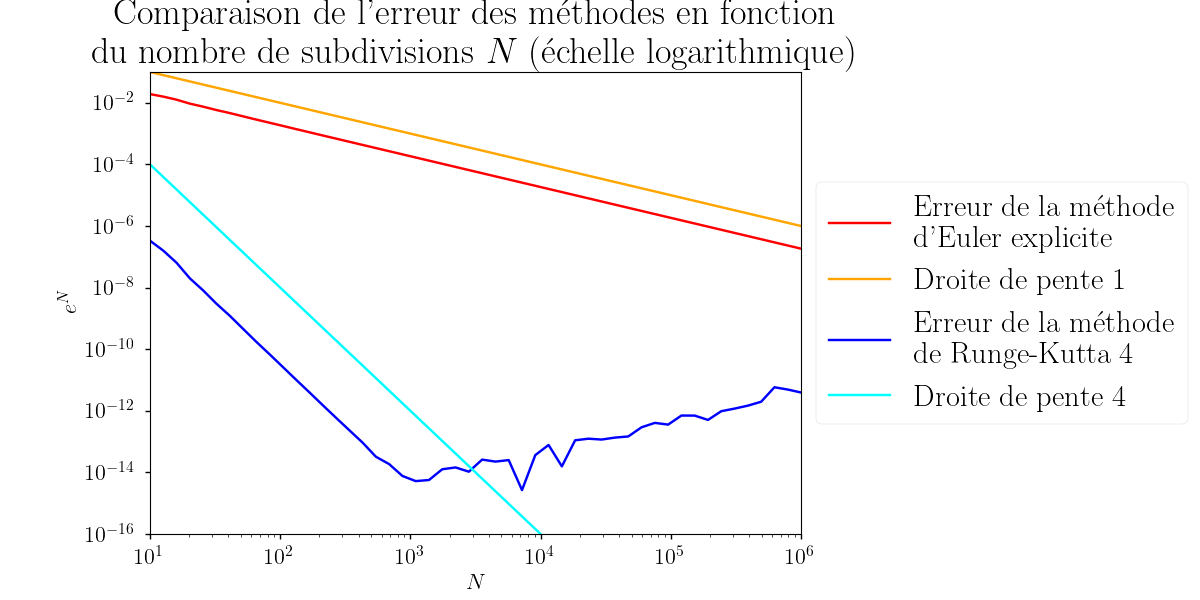
\includegraphics[width=\textwidth]{methodsError.png}
        \caption{Comparaison des méthodes en fonction de N}
    \end{center}
\end{figure}
On observe effectivement que la méthode Euler est d'ordre 1 et que la méthode de Runge-Kutta 4 est d'ordre 4. Sur le graphe de l'erreur de la méthode RK4 l'erreur dégénerre dû à l'accumulation d'erreur de précision machine car la méthode de Runge-Kutta 4 a une précision inférieure à la précision machine.

\newpage
\section{Interprétations}
Dans cette section, on illustre à l'aide de méthodes numériques les résultats de stabilité démontré précédemment.

\begin{figure}[!ht]
    \label{fig:EqAS-Dsup0}
    \centering
    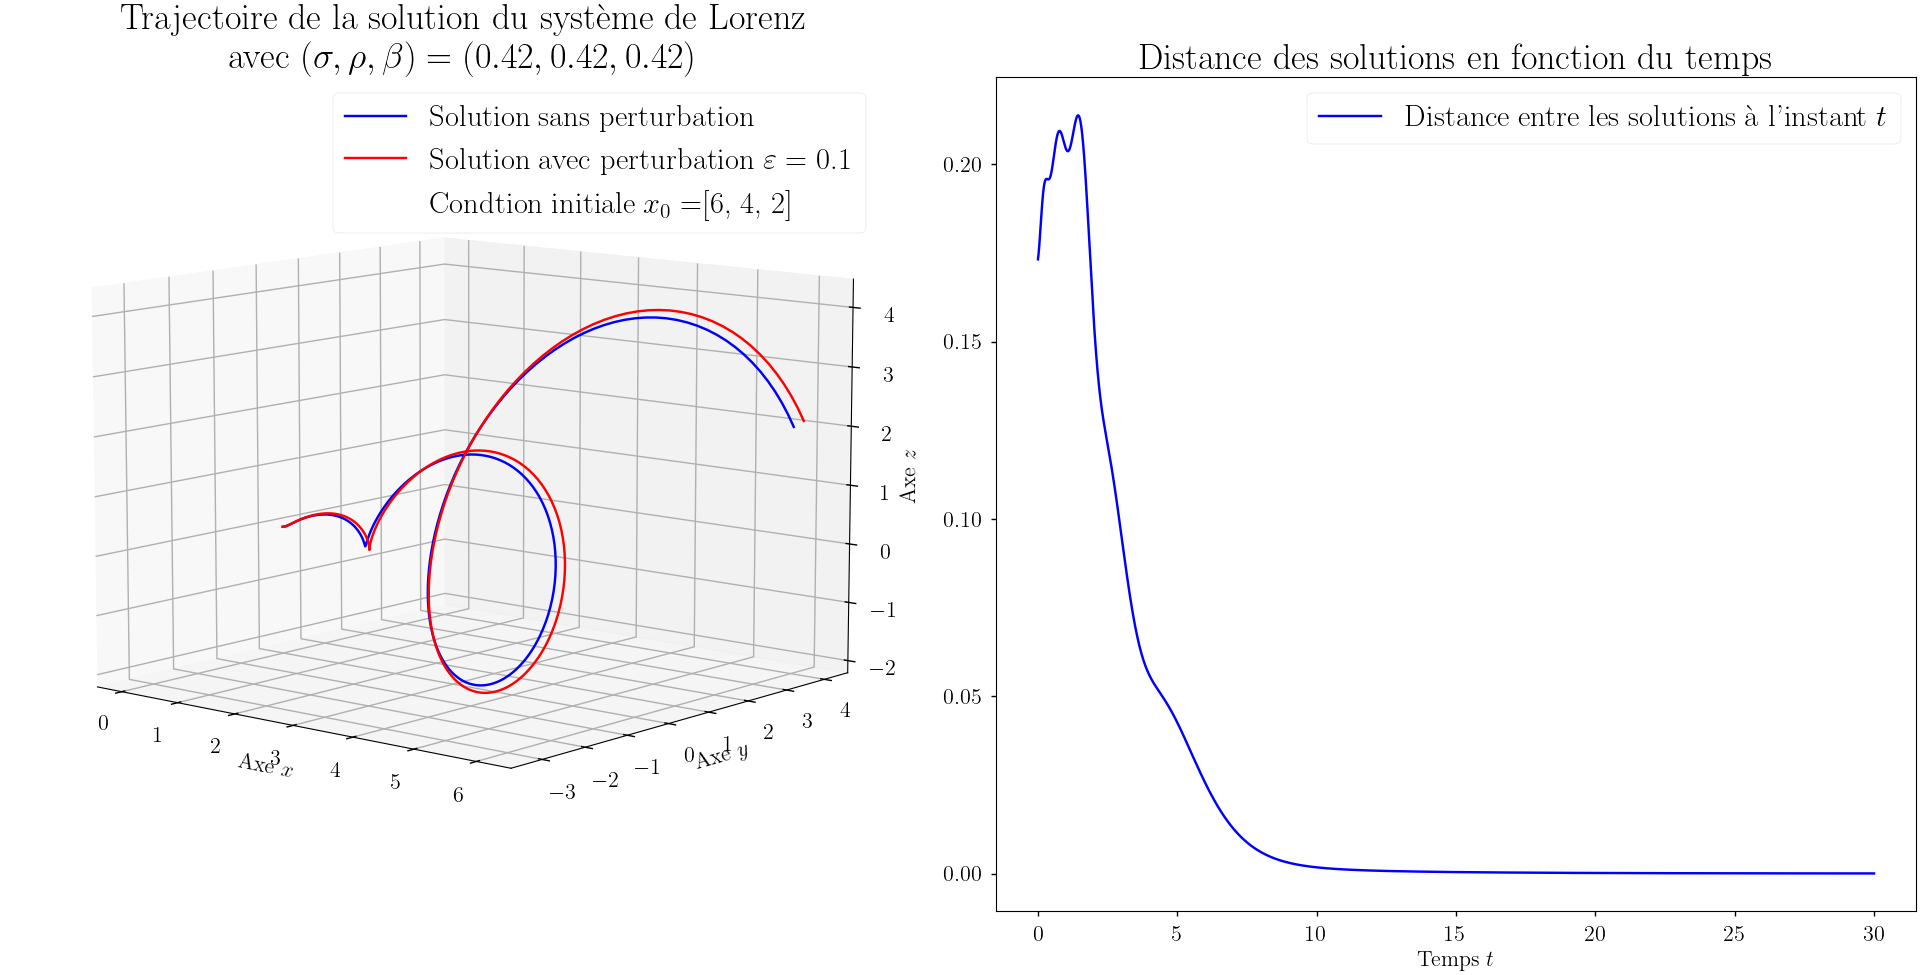
\includegraphics[width = \textwidth]{EqAS-Dsup0}
    \caption{Exemple d'équilibre assymptotiquement stable pour $\Delta>0$}
\end{figure}

\begin{figure}[!ht]
    \label{fig:EqAS-Deg0}
    \centering
    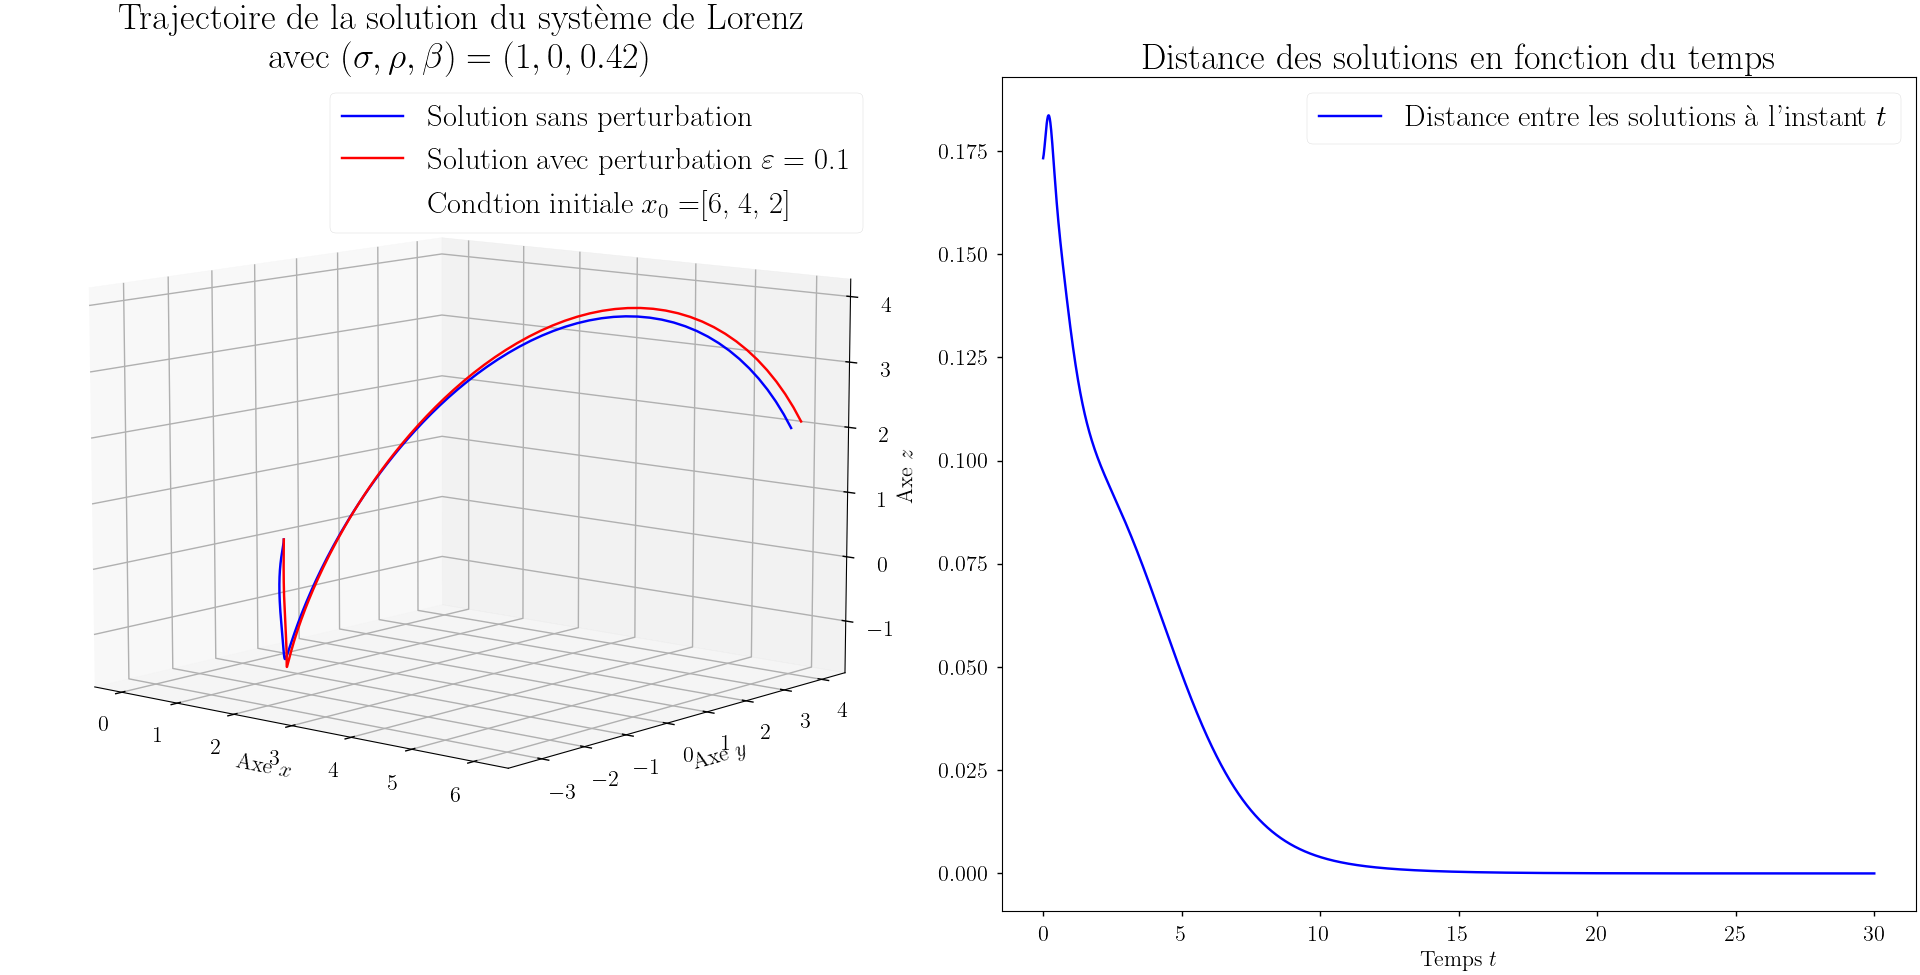
\includegraphics[width = \textwidth]{EqAS-Deg0}
    \caption{Exemple d'équilibre assymptotiquement stable pour $\Delta=0$}
\end{figure}

\begin{figure}[!ht]
    \label{fig:eqAS-Dinf0}
    \centering
    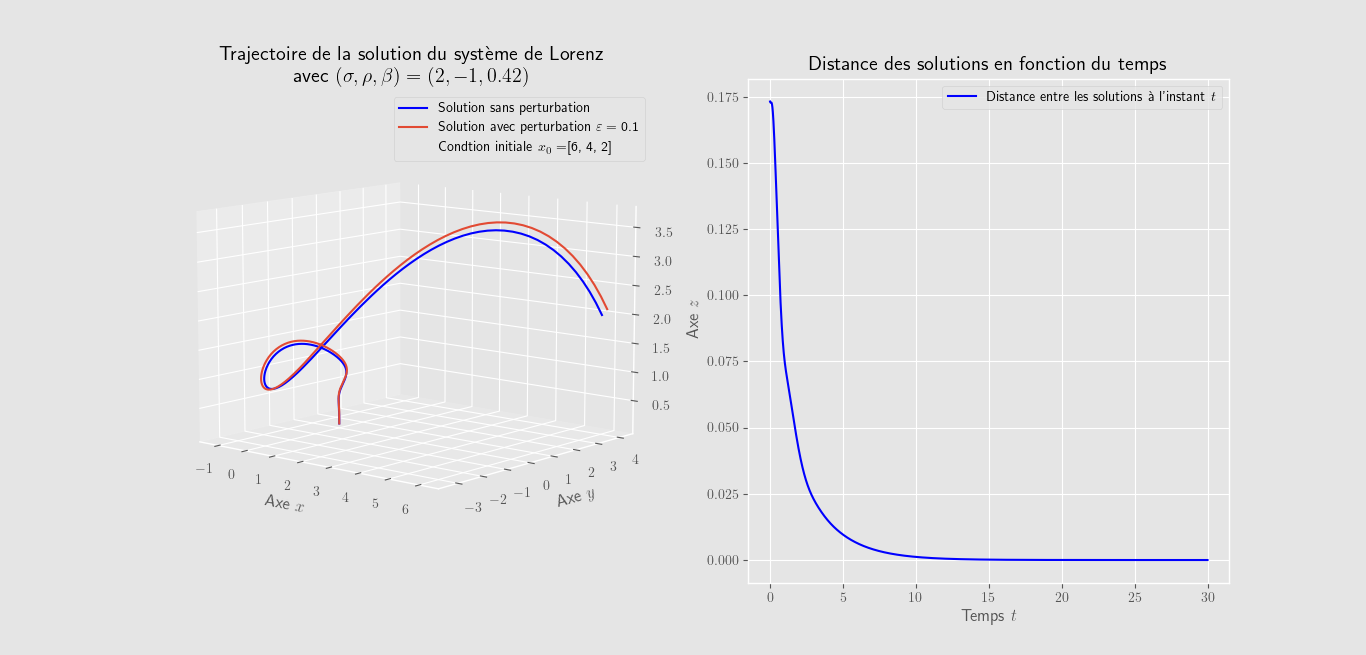
\includegraphics[width = \textwidth]{EqAS-Dinf0}
    \caption{Exemple d'équilibre assymptotiquement stable pour $\Delta=0$}
\end{figure}
Dans les figure \ref{fig:EqAS-Dsup0} ,\ref{fig:EqAS-Deg0} et \ref{fig:eqAS-Dinf0}, on observe bien que les solutions commencent leurs trajectoires avec une distance l'une de l'autre et ensuite se rapprochent jusqu'a un écart très faible. On est dans les cas des propositions respectivement \ref{prop:eqDsup0},\ref{prop:eqDeg0} et \ref{prop:eqDinf0}, cela correspond bien aux cas d'un équilibre assymptotiquement stable.

\begin{figure}[!ht]
    \centering
    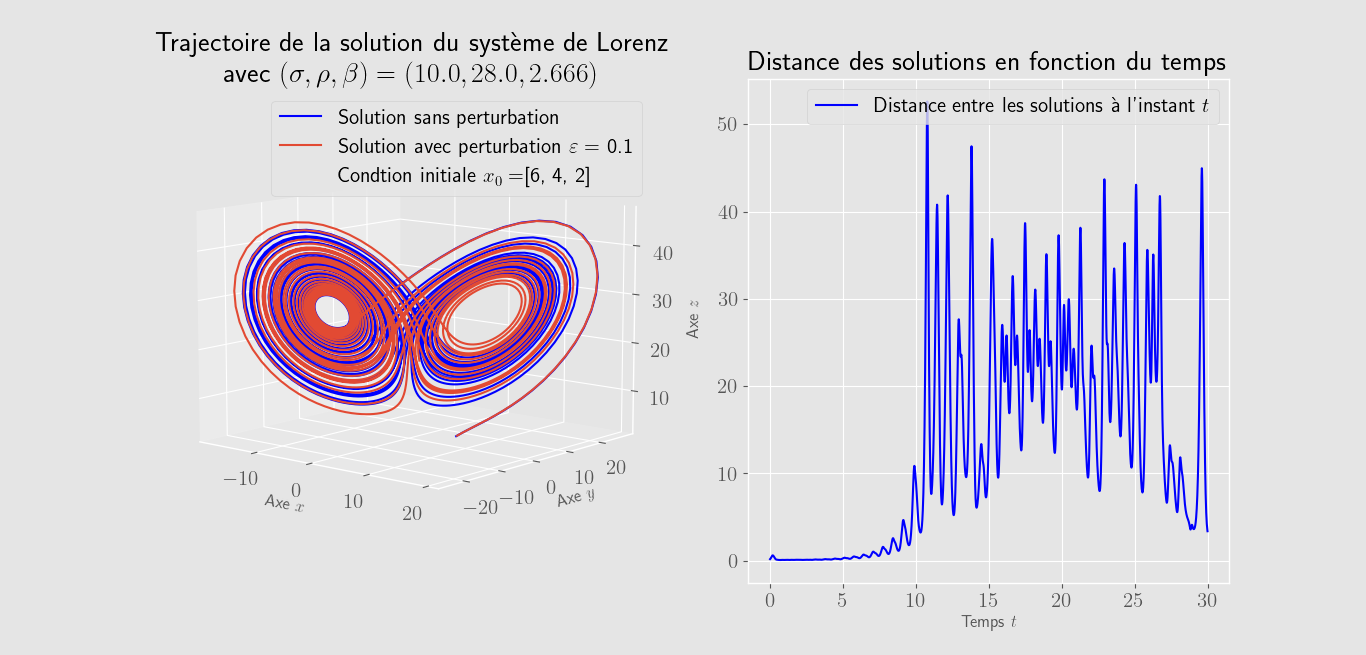
\includegraphics[width = \textwidth]{EqINS-Dsup0}
    \caption{Exemple d'équilibre instable pour $\Delta>0$}
    \label{fig:EqINS-Dsup0}
\end{figure}
Dans cette configuration (figure \ref{fig:EqINS-Dsup0}) on retombe sur les paramètres qui permettent d'observer la trajectoire en forme d'ailes de papillon décrite par E.Lorenz lors de son article de 1963 \cite{edward_n_lorenz_deterministic_1963}. La figure observée apparaît pour les paramètres $(\sigma,\rho,\beta) = (10,28,8/3)$. D'après la proposition \ref{prop:eqDsup0} c'est un équilibre instable pour \eqref{Lorenz}. Pour la période observée, on observe aucune forme de stabilisation de la trajectoire autour de $0_{\R^3}$, c'est donc bien le cas d'un équilibre instable.

\begin{figure}[!ht]
    \begin{center}
        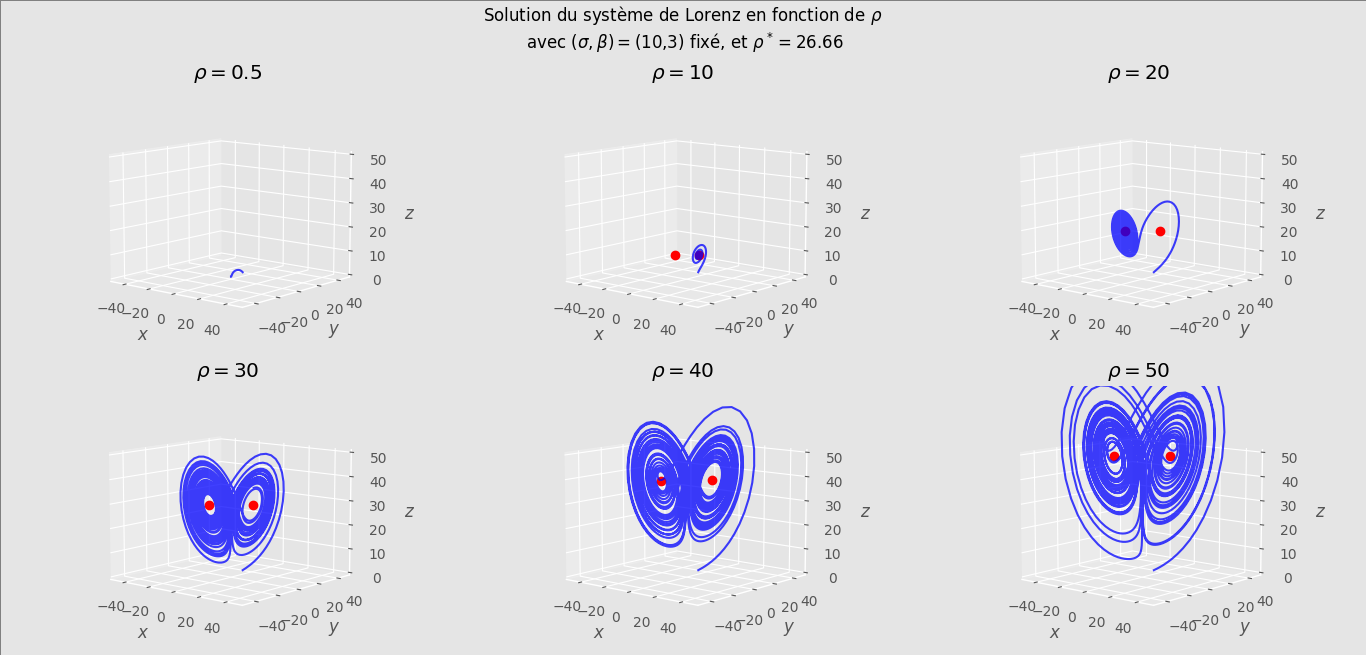
\includegraphics[height=0.73\textheight]{Eq-Spm}
        \label{fig:Eq-Spm}
        \caption{Solutions de \eqref{Lorenz} en fonction de $\rho$}
    \end{center}
\end{figure}

Dans la figure \ref{fig:Eq-Spm} on a $\rho^* \approx 26,66$, on observe alors:
\begin{itemize}
    \item pour $\rho = 1/2$, le système est très simple puisque les équilibres sont réduits à $0_{\R^3}$ de plus nous sommes dans le cas où $\Delta < 0$ et l'équilibre est assymptotiquement stable donc la solution va directement vers $0_{\R^3}$
    \item  Pour les cas $\rho = 10$ et $\rho =20$, on se retrouve dans le cas ou les équilibres existent et sont assymptotiquement stables car $\rho<\rho^*$, on observe bien que la trajectoire de la solution se rapproche d'un équilibre et ne semble pas s'en éloigner.
    \item Pour les cas restants on a, $\rho>\rho^*$ on observe alors que la trajectoire de la solution semble s'étendre dans l'espace sans jamais se diriger vers un équilibre. Cependant les solutions semblent rester dans une sous partie de l'espace.
\end{itemize}

\newpage
\section{Conclusion}

Au cours de notre étude à l'aide de l'exemple de l'attracteur de Lorenz, nous avons approché le concept de chaos dans les équations différentielles. Notre étude nous a permis de constater que les comportements singuliers proviennent de faibles perturbations dans les conditions initiales. De plus ces comportements ne sont pas uniquement inhérents aux conditions initiales. Ils dépendent de la configuration du système: nous avons pu constater qu'il existe des jeux de paramètres, donc de configurations telles que les trajectoires des solutions ne font pas apparaître de comportement chaotique. On peut faire une analogie avec la mécanique des fluides. Les systèmes à grand nombre de Rayleigh sont hautements chaotiques. \`A contrario les systèmes à faible nombre de Rayleigh ne sont pas sensibles aux faibles perturbations. C'est d'ailleurs la correspondance de $\rho$ dans les approximations de Lorenz. Ces mouvements qui pourraient sembler aléatoires sont en fait déterministes. Cependant dû à la difficulté de mesurer de manière suffisamment fiable les grandeurs qui évoluent dans le système, il en devient hautement imprévisible. C'est ce qu'on a pu constater durant l'étude des équilibres.
Pour continuer notre étude, nous pourrions chercher sous quelles conditions les trajectoires restent-elles dans une partie bornée de l'espace.
\newpage
\section{Annexes}
\subsection*{Méthode des rectangles}
\addcontentsline{toc}{subsection}{\protect\numberline{}Méthodes des rectangles}
La méthode des rectangles est une méthode numériques pour approximer le calcul d'intégrale. Elle consiste à approximer l'aire sous la courbe par un rectangle. On peut choisir la hauteur du rectangle de différentes manières, à gauche, au millieu et à droite. Comme présenté dans la figure les figures qui suivent.
\begin{figure}[ht]
    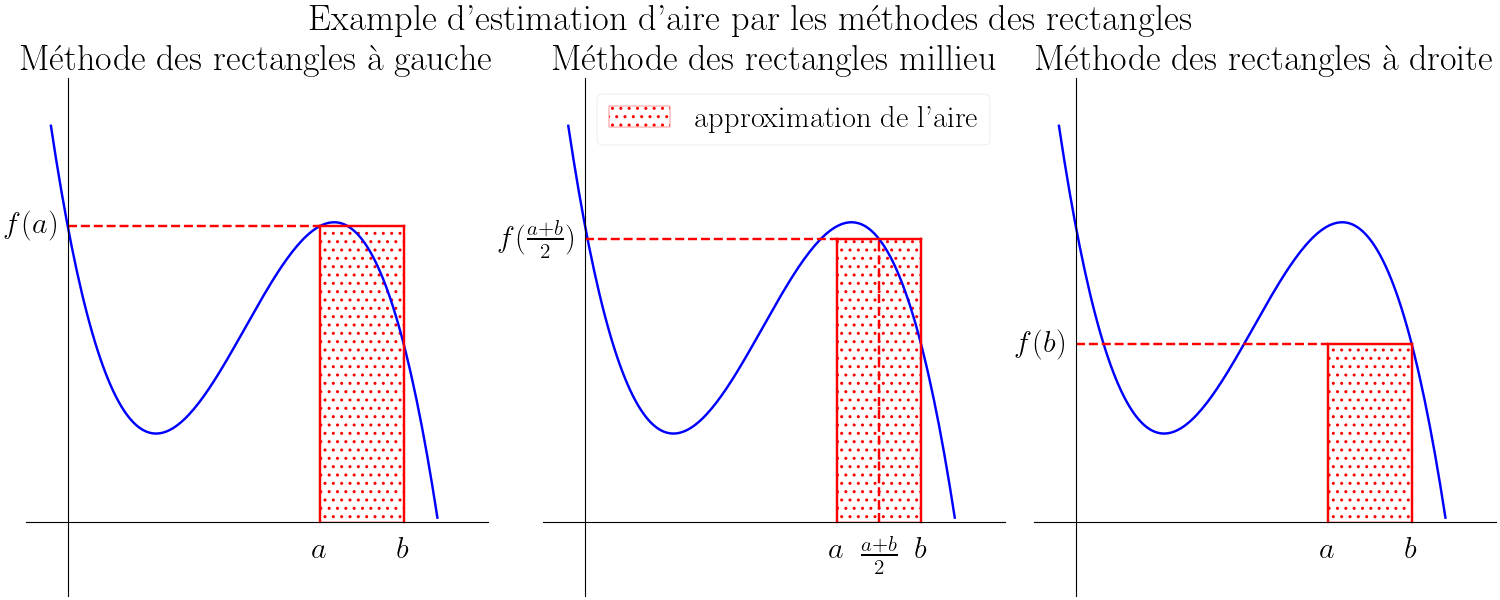
\includegraphics[width=\textwidth]{MethodeRect}
\end{figure}

Considérons l'intégrale suivante:
\[
  I := \int_a^b f(x)\ \mathrm{d}x\quad \text{avec }a<b \text{ et } f \text{ continue par morceaux}
\] 
On peur approximer cette intégrale de trois manières différentes:\\
Méthode des rectangles à gauche:
\[
    I \approx (b-a) f(a)
\]\\
Méthodes des rectangles millieu:
\[
    I \approx (b-a) f(\frac{a+b}{2})
\]\\
Méthodes des rectangles à droite:
\[
    I \approx (b-a) f(b)
\]
\begin{example}[Remarque]
    Comme le montre les images ci-dessus l'approximation peut-être grossière. Dans l'exemple de la méthode des rectangles à droite une majorité de l'aire sous la courbe n'est pas incluse dans le rectangle.
\end{example}

\subsection*{Code}
\addcontentsline{toc}{subsection}{\protect\numberline{}Code}
L'ensemble des graphes ont été génerés sur python à l'aide des bibliothèques Matplotlib et Numpy. Vous pouvez retrouver l'ensemble de ces codes sur le Github du projet ou sur filesender jusqu'au 20/06/2024:
\begin{itemize}
    \item Filesender:\\ \url{https://filesender.renater.fr/?s=download&token=8ddd43a9-c73c-4fc9-b54e-8f3845f5c640}
    \item Github:\\ \url{https://github.com/N3rida/Projet}
\end{itemize}
Les correspondance des fichiers sont celles donné par ce tableau:\\
\begin{tabular}{|m{.3\textwidth}|m{.65\textwidth}|}
    \hline
    genGraph.py & générations des graphes des exemples de la stabilité pour les différent cas de $\Delta$\\
    \hline
    GrapheSolution.py & graphe de la solution comme dans la page de couverture\\
    \hline
    DeltaDomain.py & graphe du signe de $\Delta$ en fonction de $\rho$ et $\sigma$\\
    \hline
    genSpmEquilibrium.py & graphe pour comparer l'évolution de la trajectoire autour des équilibre $S_\pm$ en fonction de $\rho$\\
    \hline
    genMethRect.py & graphe explicatif de la méthode des rectangles\\
    \hline
    methodsError & programme qui permet de comparer l'erreur entre la méthode de Euler et de Runge-Kutta 4\\
    \hline
\end{tabular}

\newpage
\nocite{*}
\printbibliography[heading=bibintoc,title={Bibliographie}]
\end{document}